\documentclass[a4paper,10pt]{article}

\usepackage[utf8]{inputenc}
\usepackage[french]{babel}
\usepackage{array,multirow,makecell}
\usepackage{color}
\usepackage{graphicx}
\usepackage{wrapfig}
\usepackage{hyperref}
\usepackage{fancyhdr}
\usepackage{fancybox}
\usepackage[squaren,Gray,cdot]{SIunits}
\usepackage{amsmath}
\usepackage{amssymb}
\usepackage{wasysym}
\usepackage{tikz}
\usepackage[tikz]{bclogo}
\usepackage{xkeyval}
\usepackage{ifthen}
\usepackage{ifpdf}
\usepackage{etoolbox}
\usepackage{mdframed}
\usepackage{xcolor}
\usepackage{tcolorbox}
\usepackage[a4paper,landscape,left=1.1cm,right=1.1cm,top=1.8cm,bottom=1.5cm]{geometry}\twocolumn
\usepackage{multicol}
\setlength{\columnseprule}{0.5pt}
\setlength{\columnsep}{25pt}

\def\d{\displaystyle}
\def\o{\overrightarrow}
\def\tr{\textcolor{red}}
\def\tb{\textcolor{blue}}
\def\tv{\textcolor{green}}
\def\tm{\textcolor{magenta}}
\definecolor{orange}{rgb}{0.99,0.69,0.07}
\definecolor{forestgreen}{rgb}{0.13,0.54,0.13}
\def\to{\textcolor{orange}}
\def\r{$\rightarrow\ $}
\def\tw{\textcolor{white}}
\def\so{\underline}
\def\su{\overline}
\def\esp{\vspace{0.2cm}}
\def\manip{\bcpanchant\ }


\newcounter{testcount} 
\newcommand{\test}{\stepcounter{testcount}
\noindent\bccrayon \textbf{\,Test \arabic{testcount}.} }

\newcounter{definitioncount} 
\newcommand{\defi}{\stepcounter{definitioncount}
\noindent\bccoeur \textbf{\,Definition \arabic{definitioncount}.} }

\newcounter{methodecount} 
\newcommand{\meth}{\stepcounter{methodecount}
\noindent\bcoutil \textbf{\,Méthode \arabic{methodecount}.} }

\setlength{\logowidth}{10pt}

\renewcommand{\theenumi}{\alph{enumi}.}
\renewcommand{\labelenumi}{\theenumi}
\renewcommand\thesection {\tr{\Roman{section} -}}
\renewcommand{\thesubsection}{\hspace{0.5cm}\tb{\arabic{subsection})}}
\renewcommand{\thesubsubsection}{\hspace{1cm}\alph{subsubsection})}

\renewcommand\bcStyleTitre[1]{\textbf{#1}}


\lhead{PCSI 2024 - 2025}
\rhead{TP physique - documents}
\chead{instruments en électricité - Sysam - Latispro}
\cfoot{\thepage}

\pagestyle{fancy}

\date{}

\begin{document}


\thispagestyle{fancy}


\begin{center}
\begin{tcolorbox}[arc=1ex, colback=lightgray, colframe=black, left=3pt, right=3pt, top=3pt, bottom=2pt]
\begin{LARGE}
\begin{center}
\textbf{Centrale Sysam - logiciel Latispro}
\end{center}
\end{LARGE}
\end{tcolorbox}
\end{center}

\section{\tr{Connexion à Latis Pro}}
  

\begin{center}
\fbox{
\begin{minipage}{10cm}
- Applications locales $\rightarrow$ Physique Chimie $\rightarrow$ Latis Pro
\esp

- Menu \textbf{Outils} $\rightarrow$ \textbf{Options} $\rightarrow$ \textbf{Type : Sysam Campus}
\end{minipage}
}
\end{center}

\section{\tr{Centrale d'acquisition Sysam - Campus}}

\noindent
• Nous utilisons la centrale d'acquisition Sysam-Campus qui peut être associée au logiciel Latis Pro ou au logiciel Oscillo 5.
\vspace{0.1cm}

\noindent
• Elle comporte 4 entrées analogiques, 4 entrées USB pour capteur et 2 sorties analogiques.

\begin{center}
\fbox{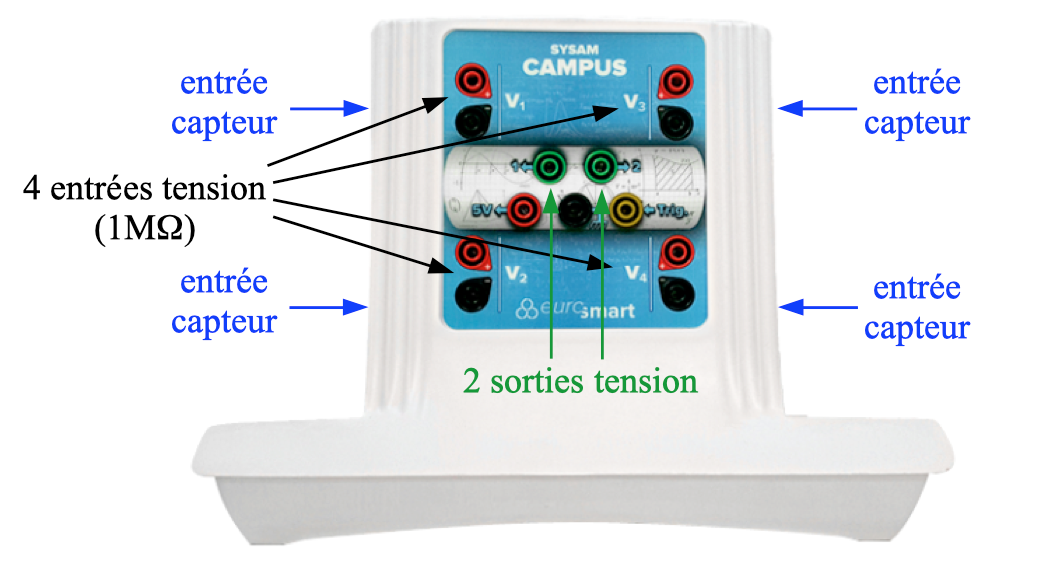
\includegraphics[scale=0.3]{sysam-image.png}} 
\end{center}

\section{\tr{Onglets Latispro}}

\noindent
• Courbes - acquisition - émission :
\begin{center}
\fbox{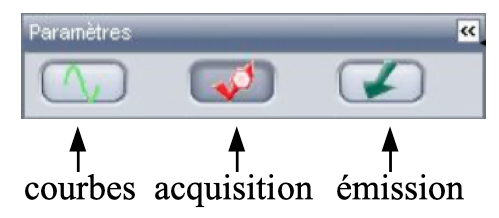
\includegraphics[scale=0.25]{latispro-image-1.png}} 
\end{center}

\noindent
• Menus :
\begin{center}
\fbox{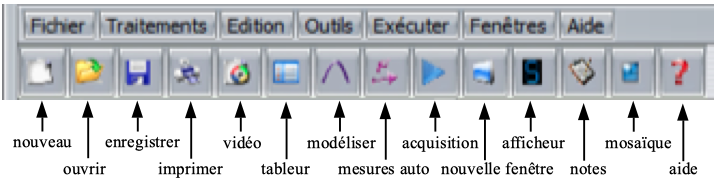
\includegraphics[scale=0.4]{latispro-image-0.png}} 
\end{center}


\section{\tr{Sorties analogiques}}

\noindent
• Pour régler les paramètres des sorties analogiques (tensions émises), cliquer sur l'\textbf{onglet émission} : 
\includegraphics[scale=0.3]{icone-emission.png} .
\esp

\noindent
• Réglages des signaux de sortie :

- émission type GBF : l'onde choisie est émise en permanence sur la sortie sélectionnée (on règle alors la fréquence, l'amplitude, ...) ;

- émission synchronisée à l'acquisition: l'onde choisie est émise en synchronisation avec l'acquisition en cours (on règle alors le nombre de période et l'amplitude paramétrées contrairement au mode précédent, l'émission débute et se termine avec l'acquisition ;

- à noter que le bouton Courbes, permet de sélectionner l'onde à émettre parmi toutes les variables du travail en cours.

\begin{center}
\fbox{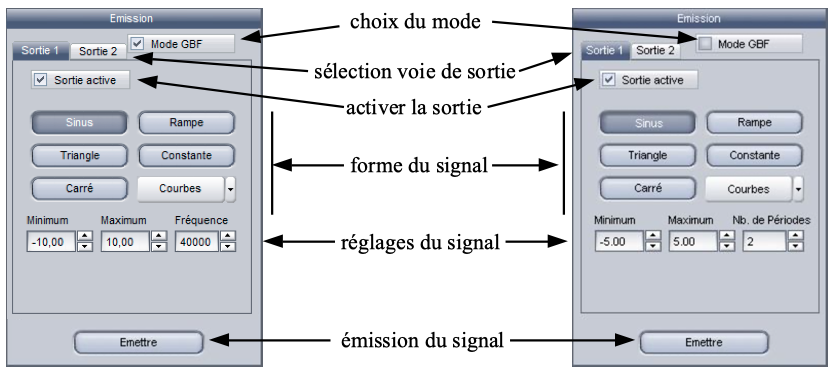
\includegraphics[scale=0.44]{latispro-image-2.png}} 
\end{center}

\section{\tr{Acquisition}}

\noindent
• Les 4 entrées analogiques ont pour caractéristiques :

\begin{center}
\begin{tabular}{|c|c|}
\hline 
calibres d'entrée & $\pm 1\ \volt$ , $\pm 10\ \volt$  , $\pm 15\ \volt$  , $\pm 30\ \volt$ \\ 
\hline 
impédance d'entrée & $1\ \mega\ohm$ \\ 
\hline 
\end{tabular} 
\end{center}

\noindent
• Pour régler les paramètres des entrées analogiques (tensions acquises), cliquer sur l'\textbf{onglet acquisition} : 
\includegraphics[scale=0.3]{icone-acquisition.png} .
\esp

\noindent
• Plusieurs modes d'acquisition sont possibles (lancée avec F10) :
\esp

\hspace{2cm}\fbox{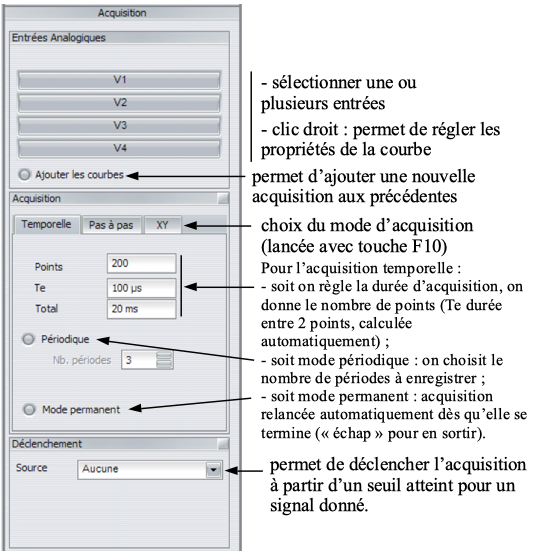
\includegraphics[scale=0.5]{latispro-image-3.png}} 
\esp

- mode Pas à pas : permet de saisir au clavier les valeurs d'une grandeur ;

- mode XY :  permet d'acquérir en temps réel deux grandeurs quelconques et de tracer l'une en fonction  de l'autre ;

- choix de $T_e$ : d'après le critère de Shannon, il faut $f_e > 2f_{max}$ ($f_{max}$ plus grande fréquence présente dans le signal étudié) donc $\d T_e < \frac{T_{max}}{2}$.

\section{\tr{Analyse des données acquises}}

\noindent
• Une fois l'acquisition faite, il est possible d'afficher les courbes, de faire des mesures sur les courbes, de les modéliser, de faire des calculs sur les données.

\subsection{\tb{Mesures sur les courbes}}

\noindent
• Cliquer sur l'\textbf{onglet Courbe} : 
\includegraphics[scale=0.3]{icone-courbe.png} .
\esp

\noindent
• Afficher les courbes : faire des cliquer-glisser sur les axes à partir de la liste des courbes.

\begin{center}
\fbox{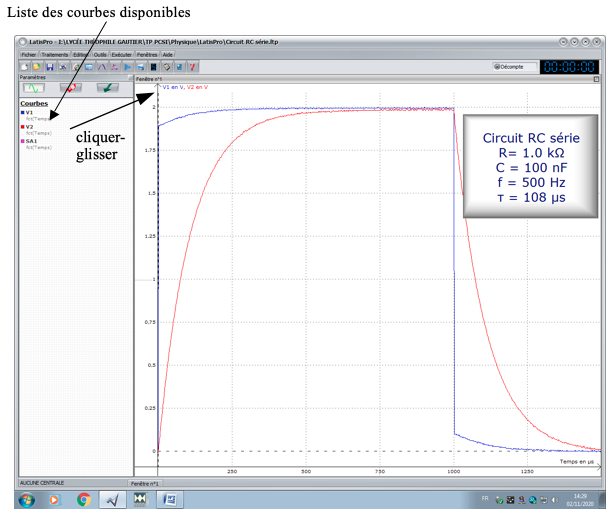
\includegraphics[scale=0.3]{latispro-image-4.png}} 
\end{center}

\noindent
• Représentation d'une courbe : clic droit sur le nom de la grandeur en haut de l'axe des ordonnées puis "Propriétés" permet :

- le choix du style (en général croix non reliées entre elles) et la couleur ;

- le choix des unités sur l'axe des abscisses et l'axe des ordonnées :

\begin{center}
\fbox{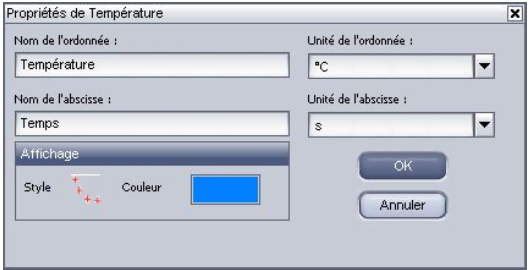
\includegraphics[scale=0.3]{latispro-image-6.png}} 
\end{center}

- le choix manuel de l'échelle (éventuellement échelle logarithmique).
\esp

\noindent
• Retirer une courbe : clic droit sur le nom de la grandeur en haut de l'axe des ordonnées puis "Retirer".
\esp

\noindent
• Mesures automatiques : dans outils ou avec l'\textbf{icône Mesures auto} puis faire un cliquer-glisser à partir de la liste des courbes.

\begin{center}
\fbox{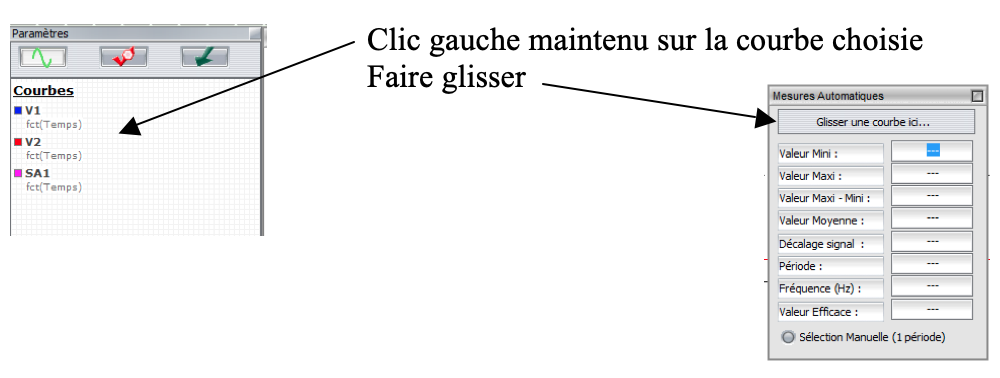
\includegraphics[scale=0.3]{latispro-image-7.png}} 
\end{center}

\noindent
• Outils sur une fenêtre graphique :

\begin{center}
\fbox{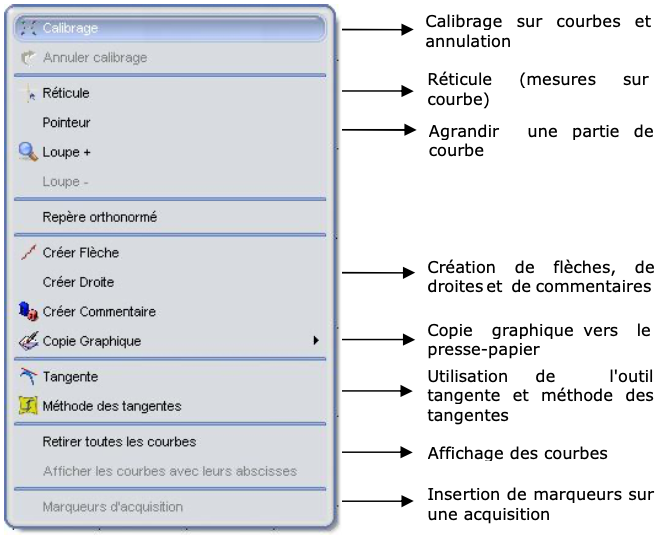
\includegraphics[scale=0.45]{latispro-image-5.png}} 
\end{center}

- "Calibrage" : dimensionne automatiquement les échelles ;
\esp

- "Réticule" : permet des mesures manuelles sur les courbes affichées :

\begin{itemize}
\item[.] mode Libre (par défaut) : le réticule se déplace librement sur la fenêtre ;
\item[.] "Lié à la courbe" : le réticule se déplace uniquement en suivant la courbe sélectionnée par le sous menu proposé ;
\item[.] "Nouvelle origine" : permet de faire une mesure entre deux points ;
\item[.] "Mesurer l'abscisse" : envoie la valeur de l'abscisse pointée vers le tableur ;
\item[.] "Mesurer l'ordonnée" : envoie la valeur de l'ordonnée principale à la liste des scalaires ;
\item[.] "Mesurer l'abscisse et l'ordonnée" ;
\item[.] "Terminer" : permet de finir le travail avec le réticule ;
\end{itemize}
\esp

- "Pointeur" : permet de modifier les points d'une courbe affichée (cliquer dessus, et le déplacer en maintenant le bouton gauche de la souris enfoncé). Les points ainsi déplacés voient leurs valeurs numériques modifiées en conséquence.


\subsection{\tb{Modélisation}}

\noindent
• Cliquer sur l'\textbf{icône modélisation} : 
\includegraphics[scale=0.2]{icone-modelisation.png} .

\begin{center}
\fbox{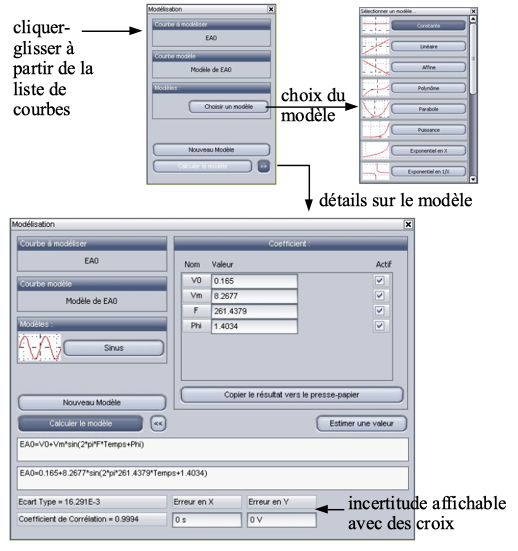
\includegraphics[scale=0.45]{latispro-image-8.png}} 
\end{center}


\subsection{\tb{Traitements des données}}

\noindent
• Calculs spécifiques : 

- le sous-menu "Calculs spécifiques" du menu "Traitements" permet d'effectuer des calculs  sur des données à l'aide d'un cliquer-glisser :

\begin{center}
\fbox{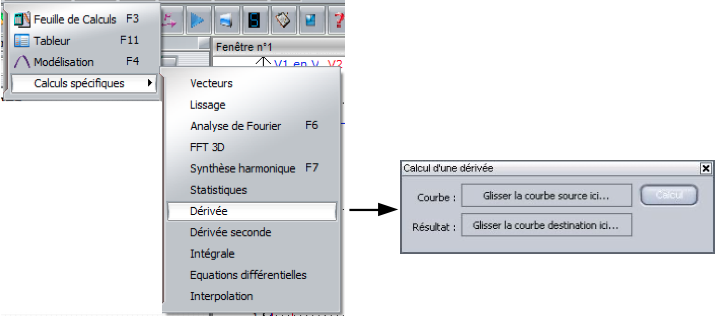
\includegraphics[scale=0.45]{latispro-image-9.png}} 
\end{center}

- "Analyse de Fourier" : permet en mode avancé d'effectuer la transformée de Fourier rapide d'un signal (on obtient son spectre).

\begin{center}
\fbox{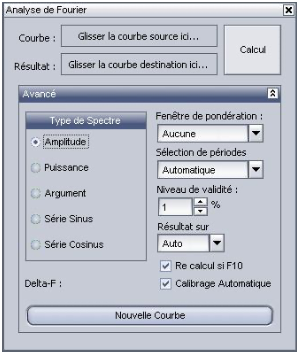
\includegraphics[scale=0.45]{latispro-image-10.png}} 
\end{center}

\subsection{\tb{Tableur}}

\noindent
• Cliquer sur l'\textbf{icône tableur} : 
\includegraphics[scale=0.3]{icone-tableur.png} .
\esp

\noindent
• Pour reporter les mesures dans une colonne, faire un cliquer-glisser de la liste des courbes vers la colonne choisie.

\begin{center}
\fbox{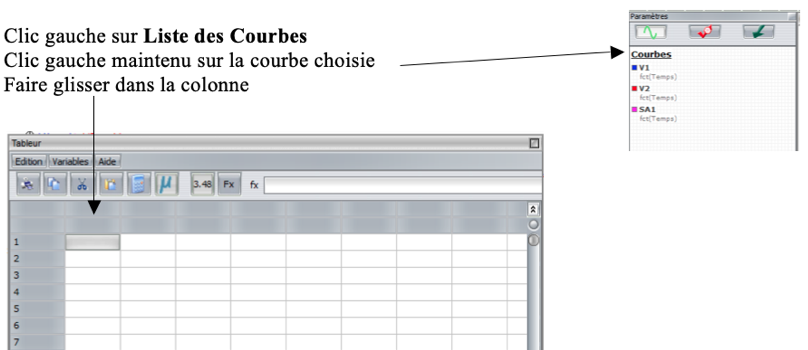
\includegraphics[scale=0.45]{latispro-image-11.png}} 
\end{center}

\noindent
• Pour créer une nouvelle variable : 

\begin{center}
\fbox{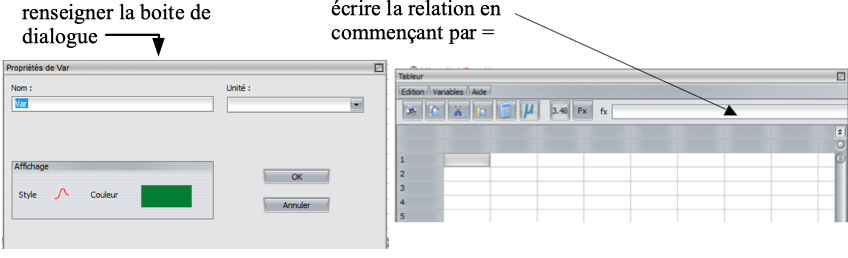
\includegraphics[scale=0.43]{latispro-image-12.png}} 
\end{center}

\noindent
• Fonctions principales disponibles :

- cos(x), sin(x), tan(x) avec x exprimé en radian ;

- sqr(x) : carré de x ; sqrt(x) : racine carré de x ;

- exp(x) : exponentielle de x ; ln(x) : logarithme népérien de x ; log(x) : logarithme décimal de x ;

- \^ : permet d’élever à la puissance ;

- deriv(x :Temps) : dérivée de x par rapport au temps.

\esp
\noindent
• Création d'une unité : 
\vspace{0.1cm}

- menu "outils" : "options" \r "superviseur" \r "gestion des unités" ;
\vspace{0.1cm}

- clic droit dans la zone "unités utilisateur", saisir le nom et le symbole (descriptif non obligatoire) et valider.



\end{document}